
\documentclass[reprint,amsmath,amssymb,aps,prc,showpacs,showkeys]{revtex4-1}


\usepackage{graphicx}
%\usepackage{dcolumn}
\usepackage{bm}
\usepackage[usenames,dvipsnames,svgnames,table]{xcolor}


\begin{document}

\newcommand{\fm}{\mbox{fm}}
\newcommand{\MeV}{\mbox{MeV}}
\newcommand{\GeV}{\mbox{GeV}}

\title{Jet Energy Loss at LHC}



\author{Vineet Kumar}
\email{vineetk@barc.gov.in}
\affiliation{Nuclear Physics Division, Bhabha Atomic Research Center, Mumbai, India}

\author{Prashant Shukla}
\affiliation{Nuclear Physics Division, Bhabha Atomic Research Center, Mumbai, India}
\affiliation{Homi Bhabha National Institute, Anushakti Nagar, Mumbai, India}

\date{\today}



\begin{abstract}
  In this work, the jet energy loss is analyzed using a monte carlo method.
  The data from LHC at $\sqrt{s_{\rm NN}}$ = 2.76 TeV and 5.02 TeV is used to extract
  the perameters for specific energy loss of jets inside QGP. Our calculations give
  good discription of the nuclear modification factor and asymmetry measurements at
  LHC.
\end{abstract}

\pacs{12.38.Mh, 24.85.+p, 25.75.-q}
\keywords{quark-gluon plasma, direct photon}

\maketitle

\section{Introduction}
\label{Sec:Introduction}


\begin{figure*}
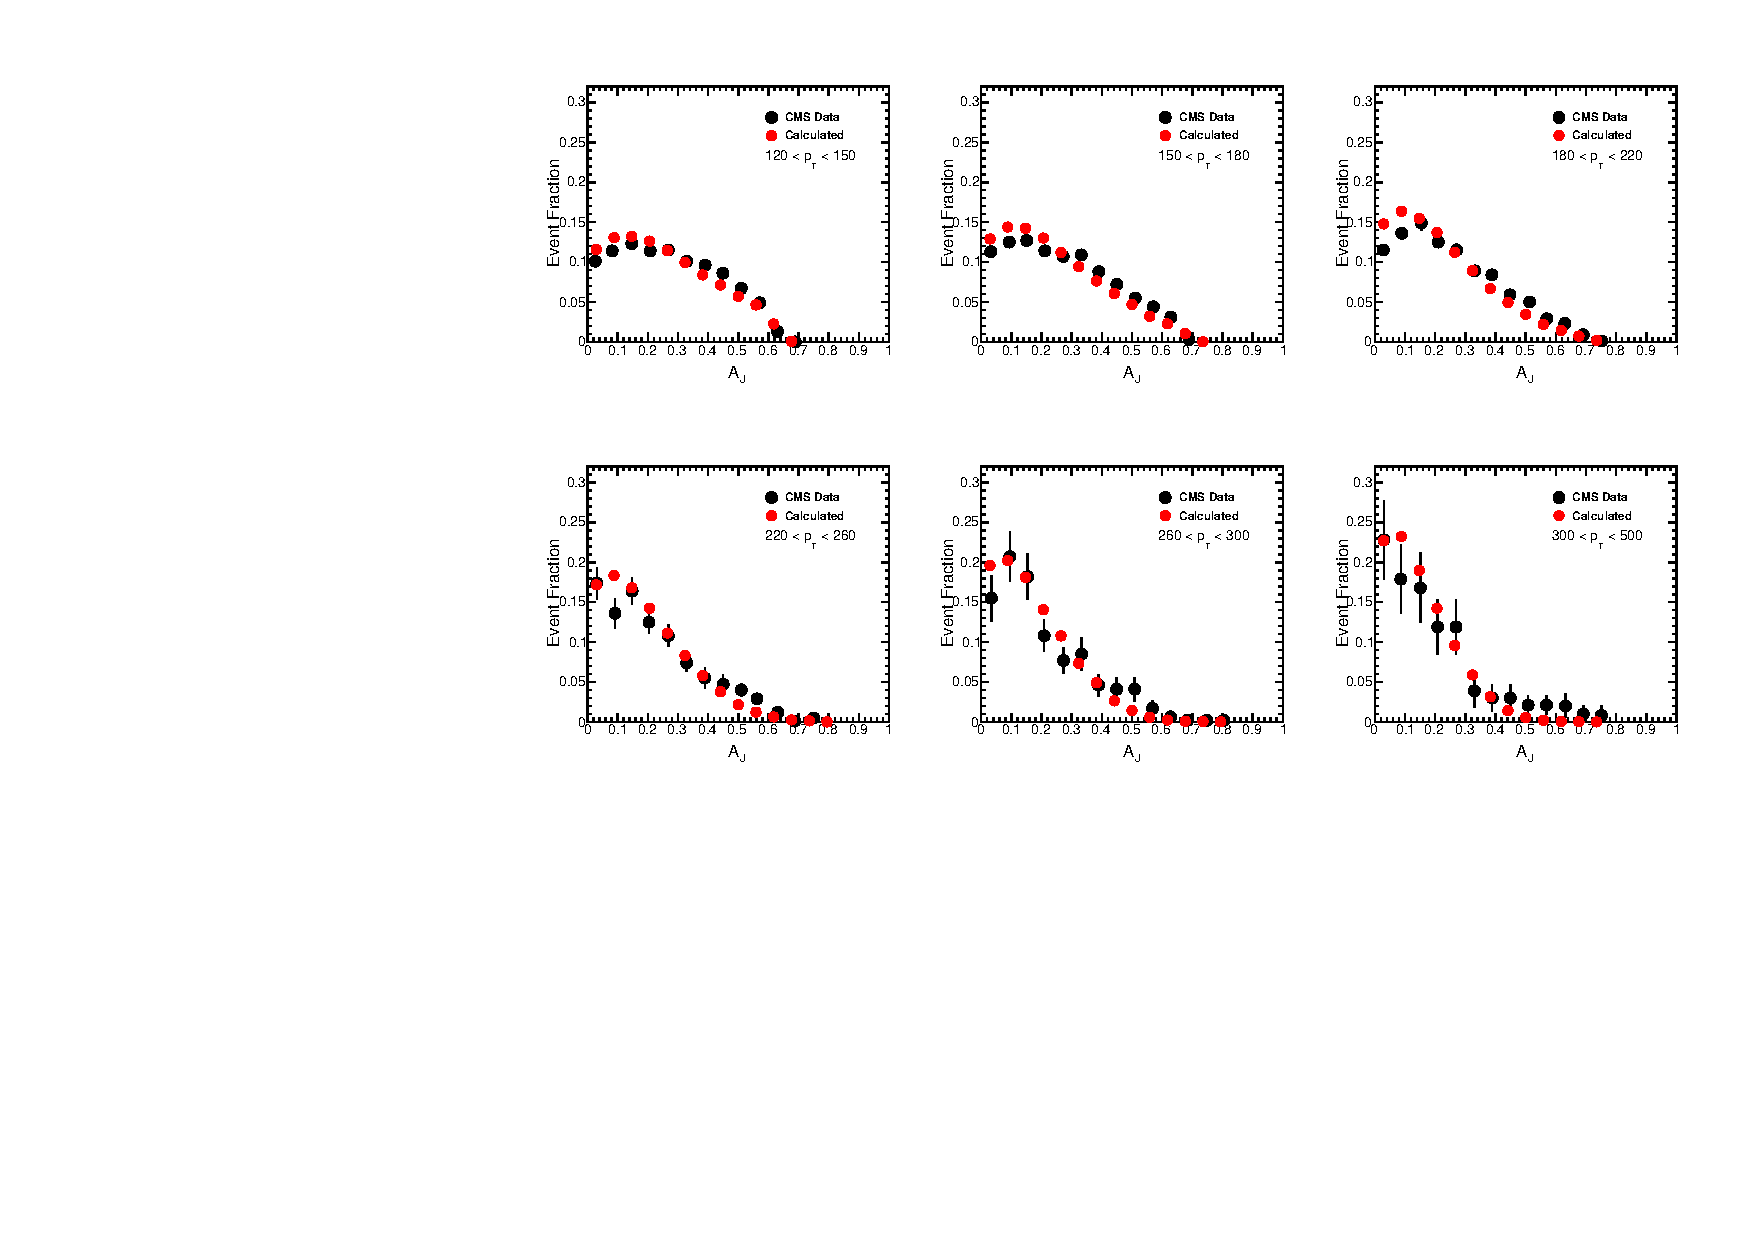
\includegraphics[width=0.99\textwidth]{Figures/Fig_Asym_DiJet_Pt.pdf}
\caption{(Color online) DiJet asymmatry measured by CMS compared with our calculations.}
\label{Fig:DiJetAsymPt}
\end{figure*}



\begin{figure*}
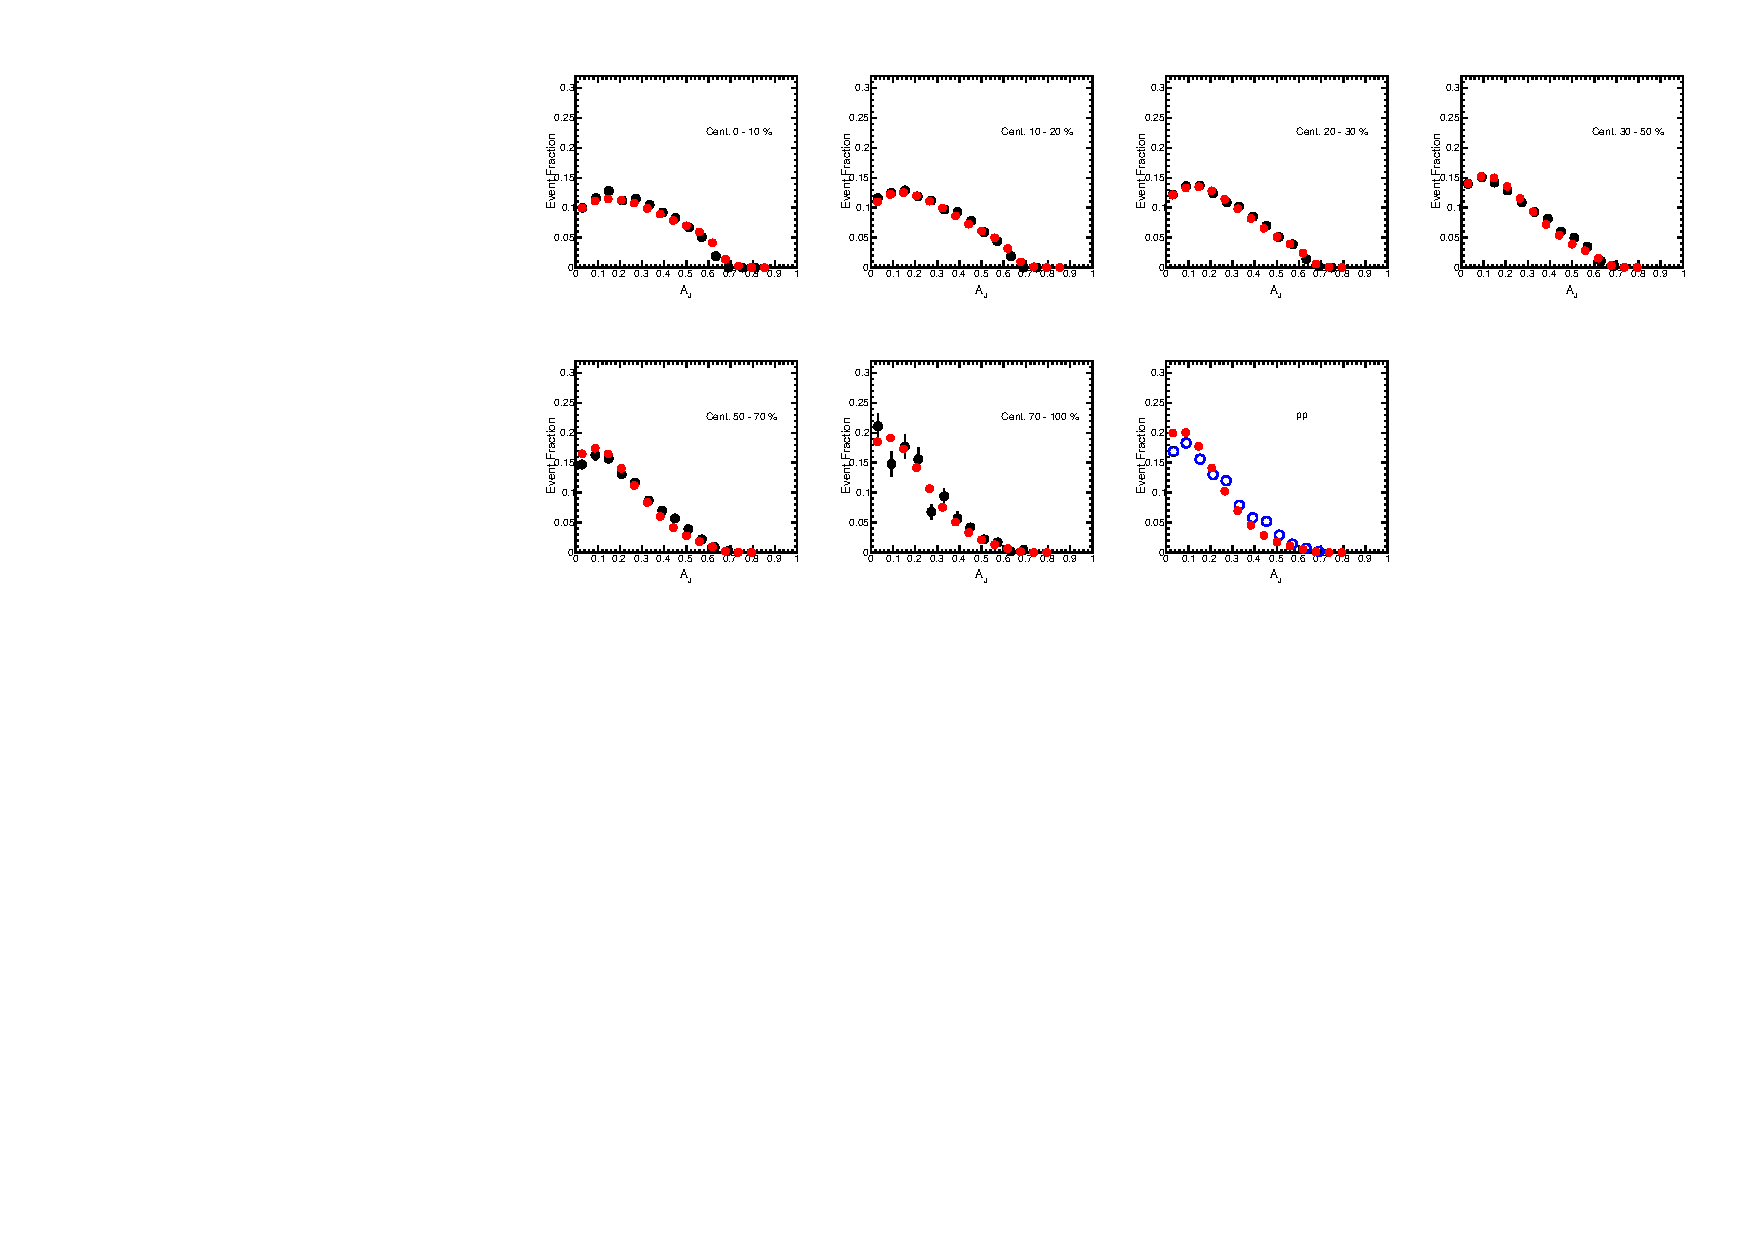
\includegraphics[width=0.99\textwidth]{Figures/Fig_Asym_DiJet_Centrality.pdf}
\caption{(Color online) DiJet asymmatry measured by CMS compared with our calculations.}
\label{Fig:DiJetAsymPt}
\end{figure*}



\begin{figure*}
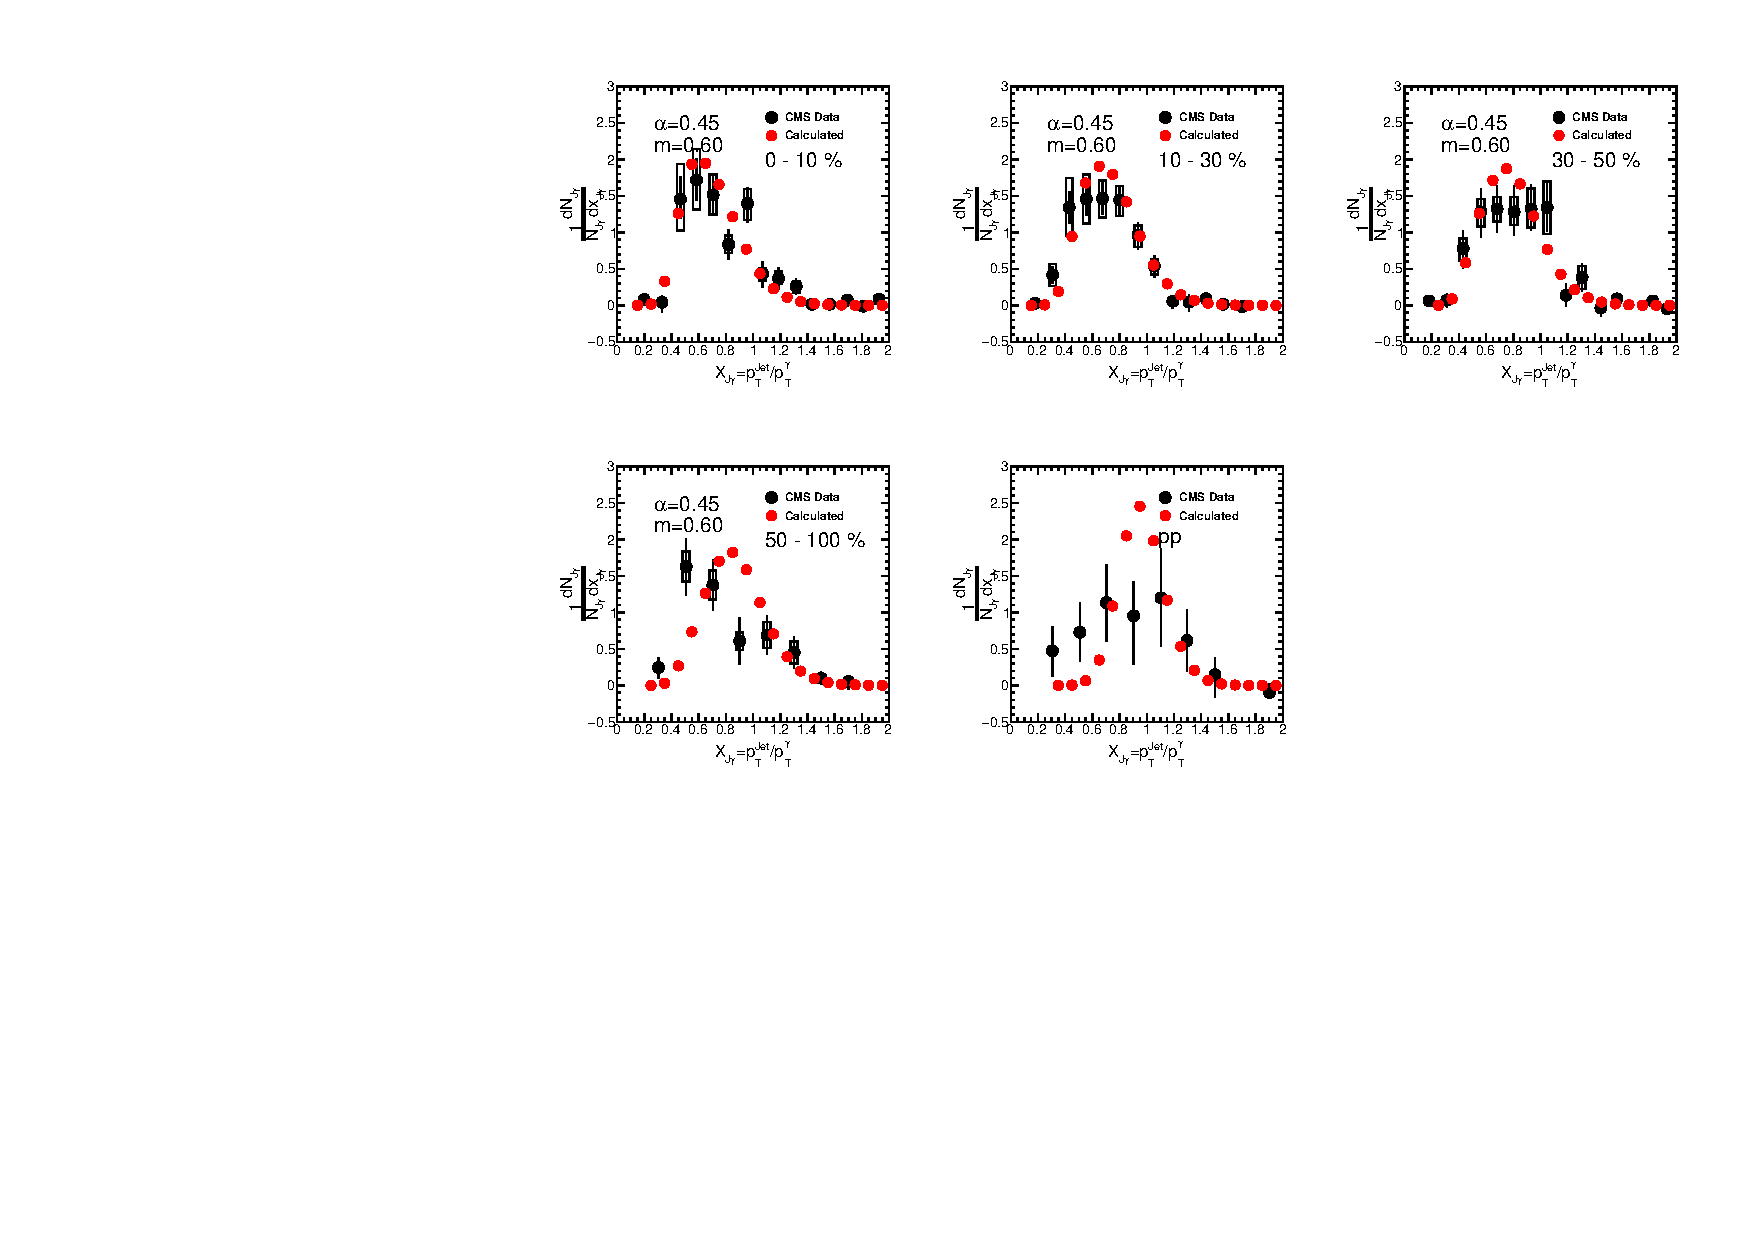
\includegraphics[width=0.99\textwidth]{Figures/Fig_XJ_GammaJet_Centrality.pdf}
\caption{(Color online) DiJet asymmatry measured by CMS compared with our calculations.}
\label{Fig:DiJetAsymPt}
\end{figure*}



\begin{figure*}
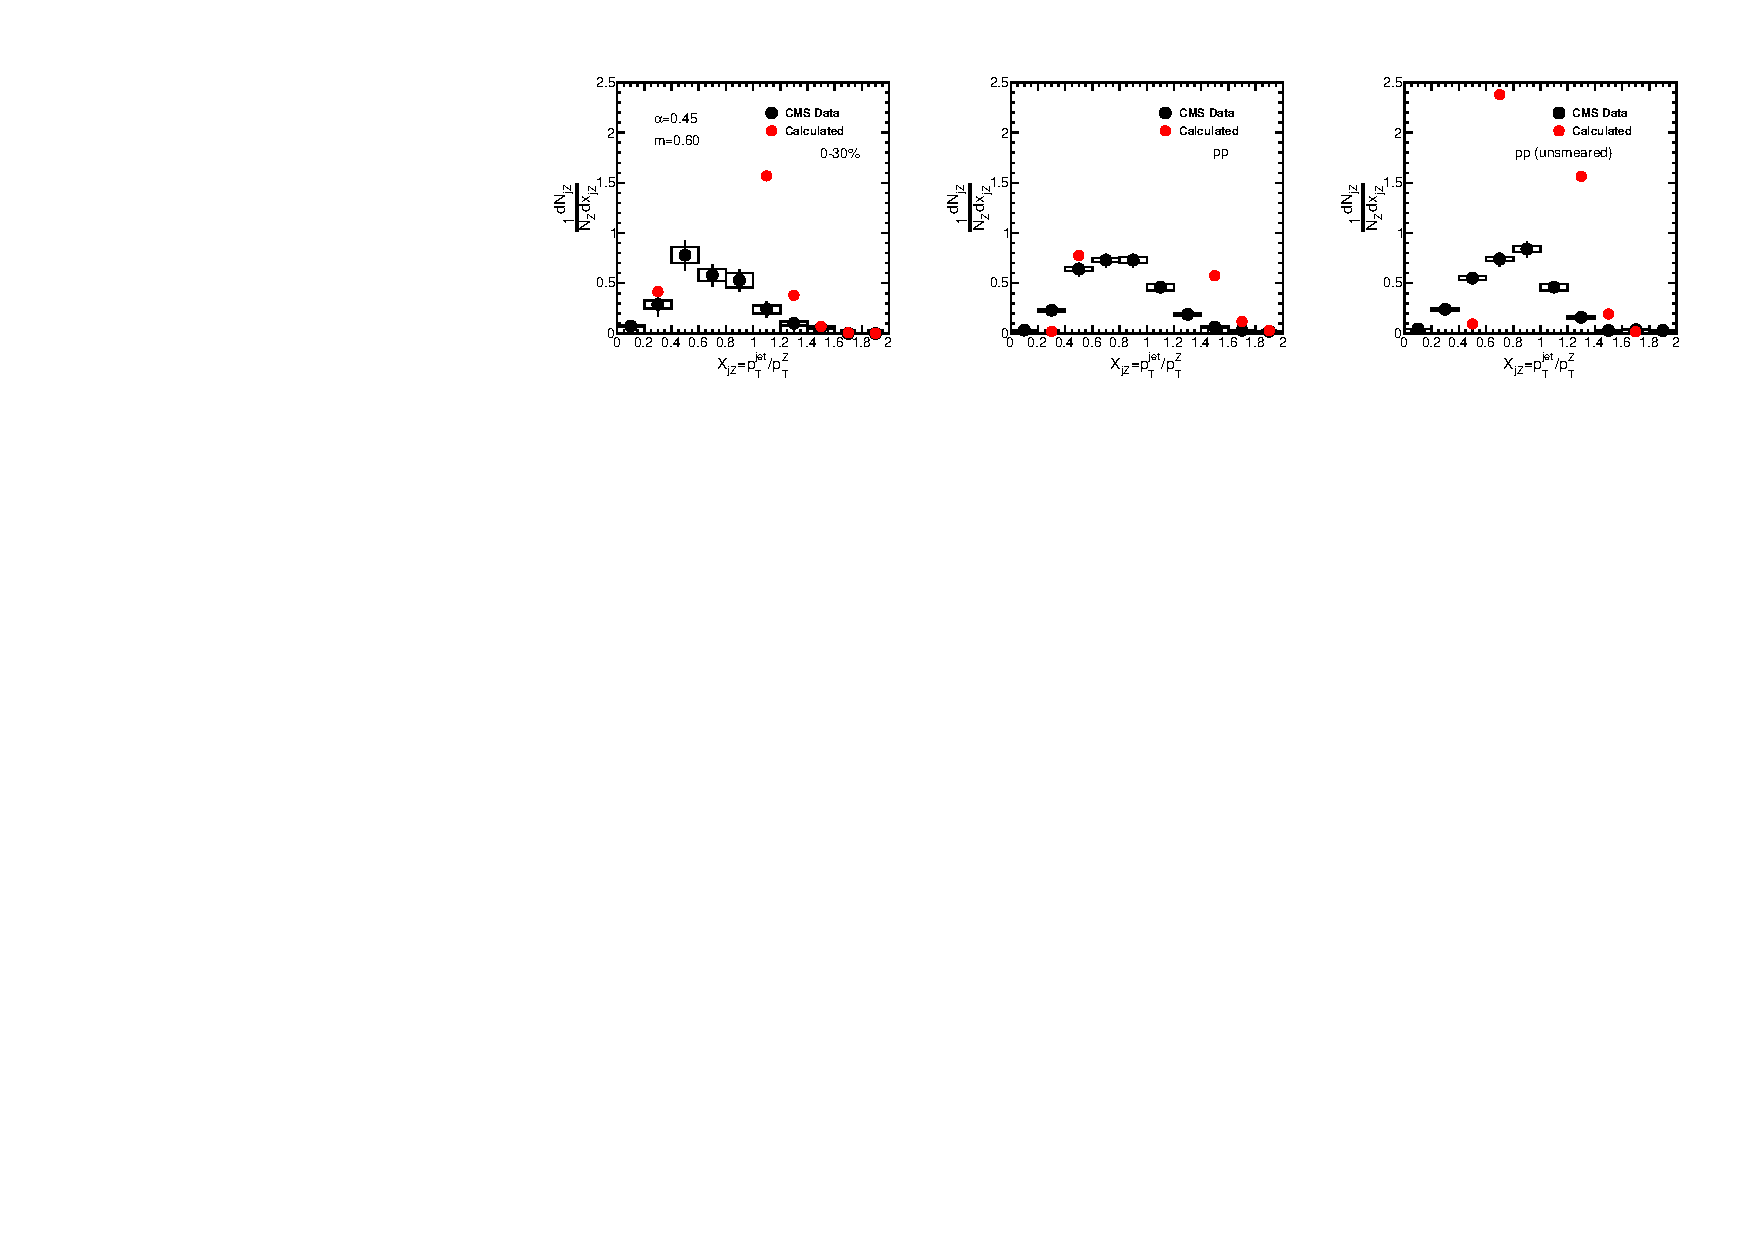
\includegraphics[width=0.99\textwidth]{Figures/Fig_XJ_Z0Jet_Centrality.pdf}
\caption{(Color online) DiJet asymmatry measured by CMS compared with our calculations.}
\label{Fig:DiJetAsymPt}
\end{figure*}



\section{Jet energy loss}
\label{Sec:JetEnergyLoss}

\section{Results and discussions}
\label{Sec:ResultsAndDiss}


\section{Summary}
\label{Sec:Summary}



\begin{thebibliography}{100}
               
\bibitem{CUTS} J. SOllfrank, P. Huovinen, M. Kataja, P.V. Ruuskanen,
             M. Prakash and R. Venugopalan, 
             Phys. Rev. C{\bf 55}, 392 (1997).

\end{thebibliography}

\end{document}




